\documentclass[nosymbols]{beamer}	% Is better for some Windows user.
\usepackage{tikz}
\usetikzlibrary{er,positioning}
\usetikzlibrary{external}

\tikzset{>=latex}
\setbeamertemplate{caption}[numbered]
\tikzstyle{every entity}=[fill=blue!20,draw=blue,thick,font=\small]
\tikzstyle{every relationship}=[fill=orange!20,draw=orange,thick,aspect=1.5,font=\small]
\tikzstyle{every attribute}=[fill=black!20,draw=black,font=\small]
\usepackage{array}
\newcommand{\PreserveBackslash}[1]{\let\temp=\\#1\let\\=\temp}
\newcolumntype{C}[1]{>{\PreserveBackslash\centering}p{#1}}
\newcolumntype{R}[1]{>{\PreserveBackslash\raggedleft}p{#1}}
\newcolumntype{L}[1]{>{\PreserveBackslash\raggedright}p{#1}}
\usepackage{pgf-umlsd}
\tikzexternalize
%
% For (excessive) usage in your document.
\newcommand{\docplace}{Magdeburg}
\newcommand{\docuniversity}{Otto-von-Guericke-University \"at Magdeburg} % Otto-von-Guericke-University Magdeburg.
\newcommand{\docuni}{OvGU}
\newcommand{\docfaculty}{Faculty of Computer Science} % Faculty of Computer Science.
\newcommand{\docfac}{INF}	% Important(!!!) for choosing the logo and colortheme. Available are:
% EIT GSE INF MATH MB MED NAT OVGU VST WW
\newcommand{\docinstitute}{Institut f\"ur Intelligent Cooperating Systems} % Department for Technical & Operational Information Systems.
\newcommand{\docinst}{ITI}
\newcommand{\docgroup}{Computational Intelligence} % Data and Knowledge Engineering Goup.
\newcommand{\docgr}{}
\newcommand{\docauthor}{Dominik Weikert}
\newcommand{\docauthoremail}{dominik.weikert@ovgu.de}
\newcommand{\doctitle}{V-REP Integrated Paparazzi Simulation} % My awesome title.
\newcommand{\doctitleshort}{Project report} % Short title.
\newcommand{\docsubtitle}{}
\newcommand{\docsubject}{Semantic Desktop}
\newcommand{\docplainkeywords}{Semantic Desktop, User Interface, Interface, Ontology, Exploration, Search} % For use in text.
\newcommand{\dockeywords}{ {Semantic Desktop} {User Interface} {Interface} {Ontology} {Exploration} {Search} } % Tagify metadata -> use package hyperref.
\newcommand{\docdate}{\today}				% Edit here author informations.
%\documentclass[nosymbols]{beamer} % Better in main.tex/Presentation.tex.
%
		% German headings.
\usepackage[T1]{fontenc}			% German typesetting.
\usepackage[utf8]{inputenc} 		%Universal/Linux Kodierung
%\usepackage[ansi]{inputenc} 		%Windows Kodierung
%\usepackage[applemac]{inputenc}	%MacOS Kodierung
%\usepackage[latin1]{inputenc} 		%Standart & Windows Kodierung
%
%\usepackage{lmodern}				% Better font encoding.
%\usepackage{verbatim} 				% Multiline Comments.
\usepackage{amsmath, amsfonts, amssymb, amsxtra} % Mathematical symbols.
\usepackage{geometry}
\usepackage{graphicx}
\usepackage{subfigure}
\usepackage{algorithm,algorithmic}
\usepackage{animate}
%
\usepackage{color}
\usepackage{xcolor}
\definecolor{EIT}{rgb}{0.498039,0.8,0.188235}
\definecolor{GSE}{rgb}{0.952941,0.439216,0.0784314}
\definecolor{INF}{rgb}{0.00392157,0.407843,0.709804}
\definecolor{MATH}{rgb}{0.819608,0.188235,0.34902}
\definecolor{MB}{rgb}{0,0.670588,0.933333}
\definecolor{MED}{rgb}{0.0627451,0.180392,0.341176}
\definecolor{NAT}{rgb}{0.2,0.709804,0.247059}
\definecolor{OVGU}{rgb}{0.454902,0,0.219608}
\definecolor{VST}{rgb}{0.54902,0.0901961,0.560784}
\definecolor{WW}{rgb}{0.341176,0.521569,0.611765}
\usecolortheme[named=\docfac]{structure}
%
\beamertemplatenavigationsymbolsempty	% Slices without navigation symbols.

\setbeamercolor*{block title example}{fg=blue!100,
bg= blue!10}
\setbeamercolor*{block body example}{fg= blue,
bg= blue!5}
\titlegraphic{
\includegraphics[height=0.12\textwidth]{include/logos/\docfac /university_token}}
\title{\doctitle}
\subtitle{\docsubtitle}
\author{\docauthor}
\institute[OvGU]{\docuniversity \\ \docfaculty} % Use it when you use the global OVGU theme or ... .
\date[Datum]{\docdate}


\setbeamertemplate{headline}% Headings
{
	\hspace*{0.02\textwidth}
	\begin{minipage}[m]{0.3\textwidth}
		\vspace*{3ex}
		
\includegraphics[height=8mm]{include/logos/\docfac /university_token}
	\end{minipage}
	\begin{minipage}[m]{0.45\textwidth}
		\vspace*{3ex}
		\doctitle 
	\end{minipage}
	\hfill
	\begin{minipage}[m]{0.14\textwidth}
		\vspace*{3ex}
		| Slide: \hfill \insertframenumber ~ / \inserttotalframenumber
		\hspace*{0.1\textwidth}
	\end{minipage}
	\color{\docfac }
	\rule{\paperwidth}{1pt}
}
%
%
%

%\setbeamertemplate{footline} % Footer
%{
%	\color{\docfac }
%	\rule{\paperwidth}{1pt}
%	\color{black}
%	\begin{minipage}[c]{\textwidth}
%		\vspace*{1ex}
%		\hspace*{0.02\textwidth} \docauthor \hfill \docdate \hspace{0.02\textwidth}
%		\vspace*{2ex}
%	\end{minipage}
%}

%
\begin{document}
%
	\addtocounter{framenumber}{-1}	% Exclude page from pagecounter.
	\begin{frame}[plain]
		\titlepage
	\end{frame}
	%
	%\setcounter{framenumber}{0}
	\frame{
		\frametitle{Overview}
		\tableofcontents
	}
	%
	
	\section{Introduction and Motivation}

\begin{frame}
	\frametitle{Project goals}
	\begin{itemize}
		\item Creation of a simulation environment for the SwarmLab copters
		\item Use existing Paparazzi infrastructure
		\item Should be easy to use and extend
	\end{itemize}
\end{frame}



\begin{frame}
\frametitle{Why do we even need a Simulation?}
\begin{itemize}
	\item Simulation allows experiments without risking potentially expensive hardware
	\item Exploration of a wide range of potential environments and conditions
	\item Scalability
\end{itemize}
\end{frame}

\begin{frame}
\frametitle{Project idea}
\begin{itemize}
	\item Idea: V-REP plugin providing communication between Paparazzi and V-REP
	\item V-REP provides the copter state, Paparazzi the corresponding commands
	\item Main advantage: same code and infrastructure usable on simulated and real copters
\end{itemize}
\end{frame}

\begin{frame}
	\frametitle{Work done in last project}
	\begin{itemize}
		\item Created basic framework
		\item Communication, control loop, coordinate transformations	
	\end{itemize}
\end{frame}

\begin{frame}
\frametitle{Goals of current project}
\begin{itemize}
	\item Implement sensors with error models, customizable from the GUI
	\item Add swarm capability and synchronization
\end{itemize}
\end{frame}

	\section{Architecture}


%\begin{frame}
%	\frametitle{Base Architecture}
%	\begin{figure}
%		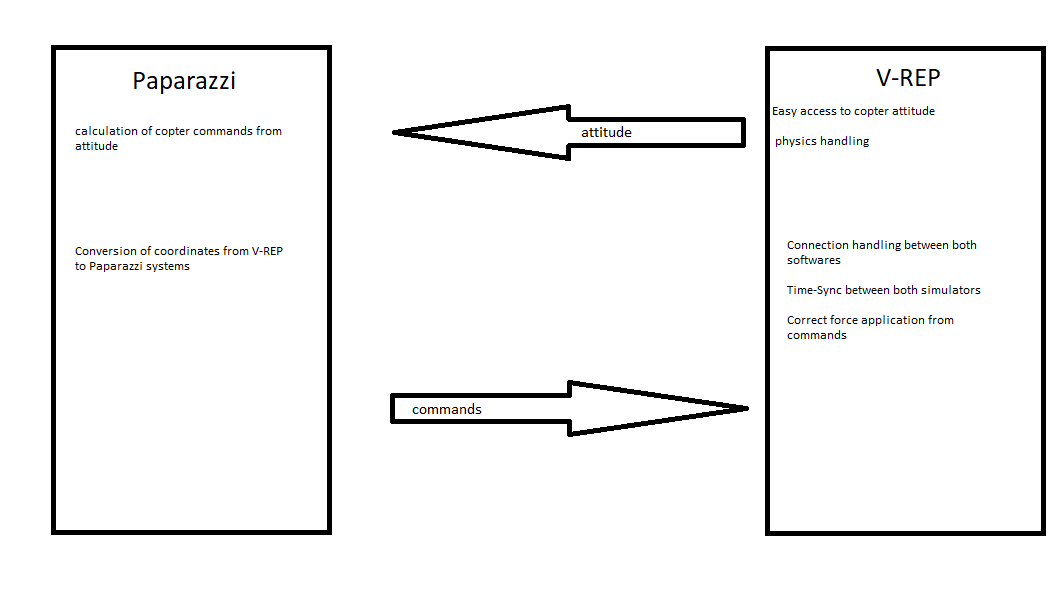
\includegraphics[width=0.9\linewidth]{graphics/expertlydrawnarchitecture}
%		\caption{Expertly drawn base architecture}
%		\footnote{make nice figure with tikzpicture, idea was to show what was provided by the programs and what i needed to add}
%	\end{figure}
%\end{frame}

\begin{frame}
	\frametitle{Base Architecture}
		\begin{center}		
			\begin{figure}
				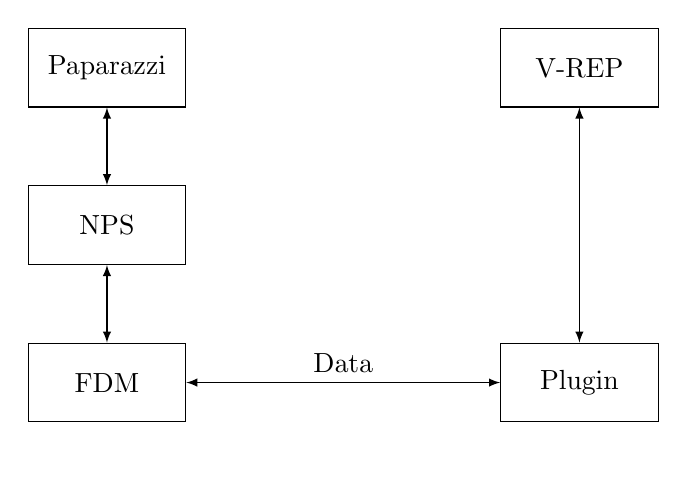
\begin{tikzpicture}[%
					basearchitecture/.pic={
						\node (pprz) at (1,5) [draw,rectangle,minimum width=2cm,minimum height=1cm]{Paparazzi};
						\node (nps) at (1,3) [draw,rectangle,minimum width=2cm,minimum height=1cm]{NPS};
						\node (fdm) at (1,1) [draw,rectangle,minimum width=2cm,minimum height=1cm]{FDM};
						\node (vrep) at (7,5) [draw,rectangle,minimum width=2cm,minimum height=1cm]{V-REP};
						\node (plugin) at (7,1) [draw,rectangle,minimum width=2cm,minimum height=1cm]{Plugin};
						\draw [<->] (pprz) -- (nps) node[midway,above left] {};
						\draw [<->] (nps) -- (fdm) node[midway,above left] {};
						\draw [<->] (vrep) -- (plugin) node[midway,above left] {};
						\draw [<->] (plugin) -- (fdm) node[midway,above] {Data};				  		  
					}			
				]
				\draw (0,0) pic {basearchitecture};
				\end{tikzpicture}
				\label{basearch}
				\caption{Basic simulation architecture}
		\end{figure}	
	\end{center}
	
\end{frame}

\begin{frame}
	\frametitle{Connection Architecture}
		\begin{tikzpicture}[%
			conarchitecture/.pic={
				\draw (1,5) rectangle (2.5,6) node[pos=.5] {nps}
				      (3,5) rectangle (4.5,6) node[pos=.5] {nps}
				      (5,5) rectangle (6.5,6) node[pos=.5] {nps}
				      (7,5) rectangle (8.5,6) node[pos=.5] {nps}
				      (9,5) rectangle (10.5,6) node[pos=.5] {nps};
		    	\draw[<->] (1.75,5) -- (1.75,3);
		    	\draw[<->] (3.75,5) -- (3.75,3);
		    	\draw[<->] (5.75,5) -- (5.75,3);
		    	\draw[<->] (7.75,5) -- (7.75,3);
		    	\draw[<->] (9.75,5) -- (9.75,3);
		    	\node[inner sep=0pt] (copter) at (1.73,2.62) { 		 	\includegraphics[width=0.175\textwidth]{graphics/finken3.png}};
		    	\node[inner sep=0pt] (copter) at (3.73,2.62) { 		 	\includegraphics[width=0.175\textwidth]{graphics/finken3.png}};		
		    	\node[inner sep=0pt] (copter) at (5.73,2.62) { 		 	\includegraphics[width=0.175\textwidth]{graphics/finken3.png}};		
		    	\node[inner sep=0pt] (copter) at (7.73,2.62) { 		 	\includegraphics[width=0.175\textwidth]{graphics/finken3.png}};		
		    	\node[inner sep=0pt] (copter) at (9.73,2.62) { 		 	\includegraphics[width=0.175\textwidth]{graphics/finken3.png}};	
		    	\draw (5,-1) rectangle (6.5,0) node[pos=.5] {V-REP};
		    	\foreach \x in {0,...,4}
		    		\draw[<->] (5.75,0) -- (1.75+2*\x,2.23);		    				
		      }
		]
		
		\draw (0,0) pic {conarchitecture};
		\end{tikzpicture}
\end{frame}

\begin{frame}
%\frametitle{Loop overview}
\begin{figure}
	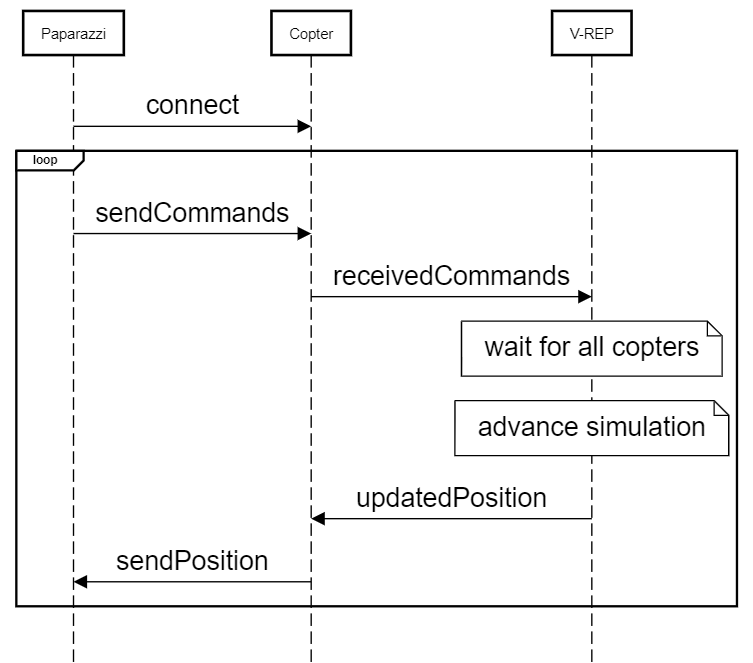
\includegraphics[height=0.88\textheight]{figures/sequence}
	\caption{Basic sync loop overview}
	\label{fig:loop}
\end{figure}
\end{frame}



\begin{frame}
\frametitle{Exchanged data: V-REP}
\begin{figure}
\scalebox{0.9}{
	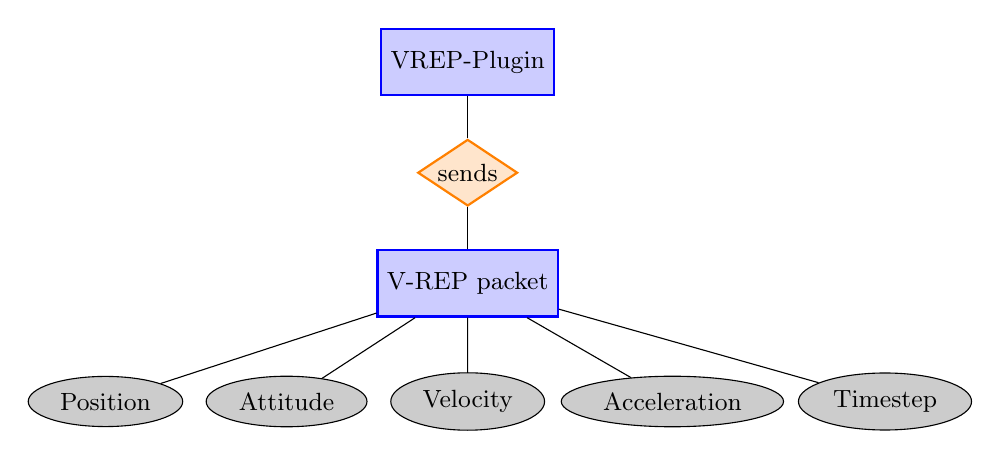
\begin{tikzpicture}[node distance=4em]
		\node[entity] (vrep) {VREP-Plugin};
		\node[relationship] (sends) [below of = vrep] {sends} edge (vrep);
		\node[entity] (packet) [below of=sends] {V-REP packet} edge (sends)
		child {node [attribute] at (-1.6,0) {Position}}
		child {node [attribute] at (-0.8,0) {Attitude}}
		child {node [attribute] {Velocity}}
		child {node [attribute] at (1.1,0) {Acceleration}}
		child {node [attribute] at (2.3,0) {Timestep}};
		
	\end{tikzpicture}
	}
\caption{Data sent by V-REP to Paparazzi}
\label{fig:vreppacket}
\end{figure}
\end{frame}

\begin{frame}
\frametitle{Exchanged data: Paparazzi}
\begin{figure}
	\scalebox{0.9}{
		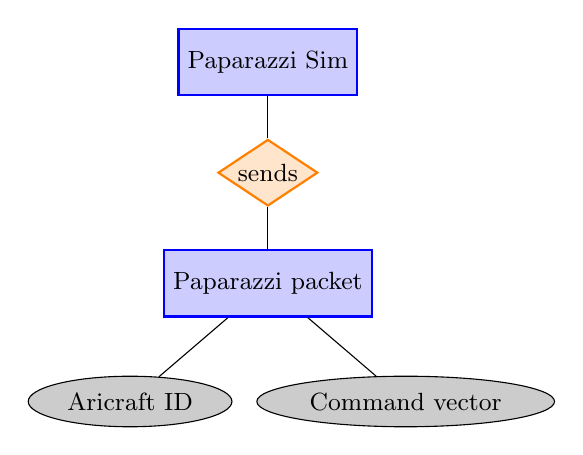
\begin{tikzpicture}[node distance=4em]
		\node[entity] (vrep) {Paparazzi Sim};
		\node[relationship] (sends) [below of = vrep] {sends} edge (vrep);
		\node[entity] (packet) [below of=sends] {Paparazzi packet} edge (sends)
		child {node [attribute] at (-1,0 ){Aricraft ID}}
		child {node [attribute] at (1,0 ){Command vector}};		
		\end{tikzpicture}
	}
\caption{Data sent by Paparazzi to V-REP}
\label{fig:paparazzipacket}
\end{figure}
\end{frame}
	\section{Problems}

\begin{frame}
\frametitle{Problems}
\begin{itemize}
	\item Connection crashing with more than one client
	\item Syncing of multiple threads for a single control thread difficult
\end{itemize}
\end{frame}



	%
	\addtocounter{framenumber}{-1}
	\begin{frame}[plain]
		
		\titlepage
	\end{frame}
%
\end{document}
